\documentclass[a4paper,fleqn,english]{book}
%
%---------------------------------------------------------------
%  LaTeX - Template, Grundlagen, Tipps, Vorlagen (Version 09)
%  (c) April 2016, Manuel Wipfli, Stefan Lisibach
%  Hochschule Luzern - Technik und Architektur
%  Abteilung Bautechnik
%---------------------------------------------------------------
%
%
%
%--------------------------------------------------------------------------------------------------------------------
% PREAMBLE
%--------------------------------------------------------------------------------------------------------------------

\usepackage{corefiles/hsluBTmaster13}

\hypersetup{%
pdfcreator={pdflatex},
pdfproducer={LaTeX},
pdftitle={UAV Serial Switch},             %%% Titel der Arbeit UNBEDINGT ANPASSEN!
pdfsubject={VA1},                         %%% Thema (subject) UNBEDINGT ANPASSEN!
pdfauthor={Stefanie Schmidiger},          %%% Autor UNBEDINGT ANPASSEN!
pdfkeywords={Aeroscout},                  %%% Stichwörter UNBEDINGT ANPASSEN!
bookmarksnumbered=true,                   %%% Nummerierte Bookmarks
bookmarksopen=true,                       %%% Bookmarks bei PDF-öffnen bereits geöffnet?
colorlinks=false,                         %%% Farbig markierte Links
plainpages=false,                         %%% zur korrekten Erstellung der Bookmarks
bookmarksopenlevel=1,												 %%% Bookmarks nur bis Hierarchiestufe Section geöffnet
pdfpagelabels,                            %%% zur korrekten Erstellung der Bookmarks
hidelinks,                                %%% Links verstecken
pdfpagelayout=TwoPageRight                %%% Voreingestellte Ansicht im PDF-Editor (z.B. Acrobat)
}%

\graphicspath{{pictures/}}                %%% Pfad, wo die Bilder abgelegt werden
\bibliography{corefiles/literatur}        %%% Datei für die Literaturquellen

%\watermark{truefirstpage} % Wasserzeichen "Entwurf": (trueall, truefirstpage,false)


%--------------------------------------------------------------------------------------------------------------------
% DOKUMENT
%--------------------------------------------------------------------------------------------------------------------

%- - - - - - - - - - - - - - - - - - - - - - - - - - - - - - - - - - - - - - - - - - - - - - - - - - - - - - - - - - 
\begin{document}													% Nicht editieren!
\lsstyle                               % Ab hier Zeichenabstand +10 (Nicht editieren!)
\fontsize{10.5}{13.7}\selectfont       % In nachfolgenden Seiten Font 10.5pt (Nicht editieren!)
\pagenumbering{alph}                   % Nötig für Richtigkeit von backref-Verweisen (Nicht editieren!)
%- - - - - - - - - - - - - - - - - - - - - - - - - - - - - - - - - - - - - - - - - - - - - - - - - - - - - - - - - - 


%--------------------------------------------------------------------------------------------------------------------
% TITELBLATT, VERSIONSTABELLE UND SELBSTSTÄNDIGKEITSERKLÄRUNG
%--------------------------------------------------------------------------------------------------------------------

\prestuffmastershort                                 % Funkt. die TB, Versionstab. und Selbstst.-Erkl. generiert
{                                                    % 1. Input kann auch selber noch angepasst werden
%\huge\textbf{\LaTeX}\\                               %%% Titel der Arbeit 1. Zeile 
%\vspace{2mm}
\huge\textbf{UAV Serial Switch\\Documentation}\\     			     %%% Titel der Arbeit 2. Zeile
%\vspace{8mm}
%\Large\textbf{bla} %%% Untertitel der Arbeit
}
{Vertiefungsmodul I}                         	       %%% Art der Arbeit
{Stefanie Schmidiger}          	      		 			%%% Autor
{Prof. Erich Styger}                          	       		%%% Advisor
{Dr. Christian Vetterli}                                   		%%% Experte
{Horw}                                          		 	%%% Ort
{2018}                                         		 		%%% Jahr XXXX
{10.01.}                                       		 		%%% Tag und Monat der Selbstständigkeitserklärung XX.XX.
{Version 0 & Initial Document & 10.01.18 & Stefanie Schmidiger}    	%%% Änderungsverzeichnis, für neue linie \\



%--------------------------------------------------------------------------------------------------------------------
% VORWORT
%--------------------------------------------------------------------------------------------------------------------

\vorwort%
{true} % ist Vorwort vorhanden? (true,false)
{% Vorwort
%
This work is being done for Aeroscout GmbH, a company that specialized in development of drones. \\
With unmanned vehicles, there are always on-board and off-board components. Data transmission between those components is of vital importance. Depending on the distance between on-board and off-board components, different data transmission technologies have to be used. \\
In this project, a hardware has been designed where multiple data inputs and outputs and multiple transmitters can be connected to a serial switch. The designed hardware features an SD card with a configuration file where data routing can be configured. \\
Data from connected devices will be collected and put into a data package with header, checksum, time stamp and other information. The package is then sent out via the configured transmitter. The corresponding second serial switch hardware receives this package, extracts and checks the payload, sends it out to the corresponding device and sends an acknowledge back to the package sender. \\
When data transmission over one transmission technology fails, the configuration file lets the user select the order of back up transmitters to be used. Data priority can also be configured because reliability of data transmission is extremely important with information such as exact location of the drone but not as important with information such as state of charge of the battery. \\
The serial switch hardware designed in the scope of this project features four serial RS232 connections where input and output devices can be connected that process or generate data. There are also four RS232 connectors where transmitters can be connected to send or receive data packages. The routing between data generating devices and transmitters to use can be done in a .ini file saved on an SD card. \\
There are two SPI to UART converters that act as the interface between the four devices connected and the micro controller respectively the four transmitters and the micro controller. \\
In a first version of the project, a Teensy 3.1 development board has been used as a micro controller unit. The software was written in the Arduino IDE with the provided Arduino libraries. As the project requirements became more complex, the limit of only a serial interface available as a debugging tool became more challenging. In the end, the first version of the software ran with more than ten tasks and an overhaul of the complex structure was necessary.\\
For this reason, an adapter board has been designed so the existing hardware could be used with the more powerful Teensy 3.5. This  adapter board features a SWD hardware debugging interface that was ready to use after removing a single component on the Teensy 3.5 development board. \\
The Teensy 3.5 was then configured to run with FreeRTOS. Task scheduler and queues provided by this operating system have been used to develop software that extracts data from received packages to output them on the configured interface or generates packages from received data bytes to send them out over the configured transmitter. The concept of acknowledges has also been applied so package loss can be detected and lost packages can be resent. \\
The software concept implemented is easy to understand, maintainable and expandable. Even though the functionality of the finished project remains the same as in the first version with Teensy 3.1 and Arduino, a refactoring has been necessary. Now further improvements and extra functionalities can be implemented more easily. } % Text des Vorworts
{Horw, January 2017} % Ort, Datum
{Stefanie Schmidiger} % Verfasser des Vorworts


%--------------------------------------------------------------------------------------------------------------------
% ZUSAMMENFASSUNG
%--------------------------------------------------------------------------------------------------------------------

\zusammenfassung%
{truedeutsch} % Ist Abstract vorhanden?(truebothsamepage, truebothseparatepages, truedeutsch, false)
{% 02_Kurzfassung
%
With unmanned vehicles, there are always on-board and off-board components. Data transmission between those components is of vital importance. Depending on the distance between on-board and off-board components, different data transmission technologies have to be used. \\
In a previous project, the hardware for a Serial switch has been designed that features four RS232 interfaces to connect data processing and generating devices and four RS232 interfaces to connect modems for data transmission. The application running on the designed base board assembled data packages with the received data from its devices and sent those data packages out to the modems for transmission. The corresponding second Serial Switch received those data packages, checked them for validity and extracted the payload to send it out to its devices.\\
A Teensy 3.2 development board acted as the main micro controller. It is a small, inexpensive and powerful USB development board for Arduino applications. The software was flexible and in its header files the user could configure individual baud rates for each RS232 interface, data routing and the use of acknowledges for data packages for each modem side. The application was running with many tasks, complex and not easy to debug because of no hardware debugging interface.\\
Then this follow up project was initiated with the aim of an application with better maintainability and expandability. The requirement for this follow up project were the use of a more powerful micro controller with Free FROS as an operating system, the use of an SD card for a configuration file and data logging and a hardware debugging interface.\\
In the scope of this project, the Teensy 3.2 was replaced with a Teensy 3.5 development board, which featured an on-board SD card slot. The Teensy 3.5 was prepared for hardware debugging and an adapter board to use the new Teensy 3.5 with the on-board headers meant for the Teensy 3.2 was designed. This adapter board allowed the use of the same base board as was designed in the previous project.\\
For the Teensy 3.5 application, the concept with data packages is applied as well and the same configuration parameters are used. The configuration is read from an .ini file saved on the SD card.\\
The functionality of the application remains the same as in the Teensy 3.2 software but with better maintainability and an easier software concept with less tasks. Hardware debugging is now possible which is of vital importance for this application to be further expandable.\\
The Teensy 3.2 application was neither well documented nor running stable. While the Teensy 3.5 application provides the same functionalities as the previous software, all its issues are documented and possible workarounds are suggested. Data handling and data loss in case of unreliable data transmission channel is handled better and the application is running stable.} % Text der Kurzfassung in Deutsch
{} % Text der Kurzfassung in Englisch

%--------------------------------------------------------------------------------------------------------------------
% INHALTSVERZEICHNIS (automatisch generiert)
%--------------------------------------------------------------------------------------------------------------------

%- - - - - - - - - - - - - - - - - - - - - - - - - - - - - - - - - - - - - - - - - - - - - - - - - - - - - - - - - - 
% outsource_TOC
%- - - - - - - - - - - - - - - - - - - - - - - - - - - - - - - - - - - - - - - - - - - - -
\clearpage
\frontmatter      % Beginn der römischen Seitenzahlen
\pagestyle{fancy}       % Für nachfolgende Seiten
\markboth{Inhaltsverzeichnis}{}
\chapter*{Table of Contents} 
\pdfbookmark[1]{Inhaltsverzeichnis}{Inhaltsverzeichnis}
\vspace{-12.8mm}
\makeatletter
\@starttoc{toc}    % Generieren des Inhaltsverzeichnisses
\makeatother
%- - - - - - - - - - - - - - - - - - - - - - - - - - - - - - - - - - - - - - - - - - - - - 	% Nicht editieren!
%- - - - - - - - - - - - - - - - - - - - - - - - - - - - - - - - - - - - - - - - - - - - - - - - - - - - - - - - - - 


%--------------------------------------------------------------------------------------------------------------------
% BEGINN DER NUMMERIERTEN KAPITEL
%--------------------------------------------------------------------------------------------------------------------

%- - - - - - - - - - - - - - - - - - - - - - - - - - - - - - - - - - - - - - - - - - - - - - - - - - - - - - - - - - 
\mainmatter%         	% Nicht editieren!
\pagestyle{fancy}%	% Nicht editieren!
%- - - - - - - - - - - - - - - - - - - - - - - - - - - - - - - - - - - - - - - - - - - - - - - - - - - - - - - - - - 
\chapter{Introduction}
% 023_Introduction
%
This work is being done for Aeroscout GmbH, a company that specialized in development of drones. \\
With unmanned vehicles, there are always on-board and off-board components. Data transmission between those components is of vital importance. Depending on the distance between on-board and off-board components, different data transmission technologies have to be used. \\
So far, each device that generates or processes data was directly connected to a modem. This is fine while the distances between on-board and off-board components does not vary significantly. But as soon as reliable data transmission is required both in near field and far field, the opportunity of switching between different transmission technologies is vital. When data transmission with one modem becomes unreliable, an other transmission technology should be used to uphold exchange of essential information such as exact location of the drone.\\
The goal of this project is to provide a flexible hardware that acts as a switch between devices and modems. Data routing between all connected devices and modems should be configurable and data priority should be taken into account when transmission becomes unreliable.\\
It should be possible to transmit the same data over multiple modems to reduce the chance of data loss for vital information. At receiving side, this case should be handled so the original information can be reassembled correctly with the duplicated data received. In case of data loss or corrupted data, a resend attempt should be started.\\
The configuration should be read from a file on an SD card. This SD card should also be used to store logging data. The system should run with Free RTOS and have a command/shell interface. When no devices are connected, the Free RTOS should go into low power mode.\\
Data loss should be handled and encryption and interleaving should be implemented for data transmission.\\
A hardware should be designed that is ready for field, with a good choice of connectors, small and light weight.\\ 
\\
It was not necessary to start from scratch for this project. Andreas Albisser has already developed a hardware with four RS-232 interfaces to connect different data generating and processing devices and four RS-232 interfaces to connect modems. As a micro controller he used the Teensy 3.2, a small, inexpensive and yet powerful USB development board that can be used with the Arduino IDE.\\
Andreas Albisser also developed a software for the designed UAV Serial Switch base board. The software concept implemented became more complex as the requirements were expanded during development. The finished product did not fulfill all requirements of Aeroscout GmbH. Therefore this follow up project was initiated with new requirements and the hope of a better and easier expandable software as an outcome.\\
Not all requirements can possibly be implemented within one semester, but good ground work should be provided for further modifications and expansions.\\
Because encryption requires a more powerful micro controller than has been used by Andreas Albisser, some hardware modifications are required in the scope of this project. The most profund change is the micro controller and usage of Free RTOS. This will therefore be the main focus inside the project. The aim is to have a stable application with at least as many features and working configuration parameters as the old software had.\\
Some requirements demand hardware changes on the base board so an evaluation needs to be done inside this project to decide how to proceed and where to invest time.\\
A detailed task description can be found in chapter two. An overview and critical analysis of the hardware and software provided by Andreas Albisser is in chapter three. In chapter four, all hardware changes that have been done in the scope of this project are described, followed by chapter four with a description of the software developed. Chapter six is for the conclusion and lessons learned.
%
\chapter{Task Description}%
% Starting Situation
%
This project has been done for the company Aeroscout. Aeroscout specialized in the development of drones for various needs. \\
With unmanned aerial vehicles, the communication between on-board and off-board devices is essential and a reliable connection for data transmission is necessary. While the drone is within sight of the control device, data can be transmitted over a wireless connection. With increasing distances, other means of transmission have to be selected such as GPRS or even satellite.\\
So far, the switching between different transmission technologies could not be handled automatically. The data stream was directly connected to a modem and transmitted to the corresponding receiver with no way to switch to an other transmission technology in case of data transmission failure. A visualization of this set up can be seen from \autoref{Old Setup}\\
\spicH{PreviousHwSetup.png}{Previous system setup for data transmission}{\label{Old Setup}}%
The aim of this project is to provide a solution that provides the needed flexibility. The finished product should act as a serial switch with multiple input/output interfaces for connecting devices and sensors and multiple interfaces for connecting transmitters. When one transmission technology fails to successfully transmit data, an other technology can be chosen for the next send attempt. Also, multiple sensors or input streams should be able to send out data over the same wireless connection. A visualization of this set up can be seen in \autoref{New Setup}\\
\spicH{NewHwSetup.png}{New system setup for data transmission}{\label{New Setup}}%
There are various kinds of information exchanged between drone and control device such as state of charge of the battery, exact location of the drone, control commandos etc. Some information such as the exact location of the drone should be prioritized over battery status information when data transmission becomes unreliable. The finished product should therefore take data priority into account. \\
Encryption should be configurable individually for each interface in case sensitive data is exchanged over a connection. \\
The finished product should be have a debugging interface such as SWD and a shell/command line interface. During run time, the software should log system data and any other relevant information to a file saved on an SD card. The SD card should also contain a configuration file so the behavior of the hardware can be changed easily. \\
A detailed description of all the requirements can be taken from the appendix Aufgabenstellung \todo{Link zur Aufgabenstellung im Appendix}.%
%
\chapter{Starting Situation}%
% Existing Work
%
%
It was not necessary to start from scratch for this project. \\
In the beginning of 2017, Andreas Albisser has already started with an implementation and provided a first solution. \\
He developed a hardware that was used as the interface between input/output data and modem for wireless transmission. He chose the Teensy 3.1 development board as a micro controller and worked with the Arduino IDE and Arduino libraries. \\
There are various problems still with his work which lead to this follow up project to improve the overall functionality.\\
More details about the work Andras Albisser has done can be taken from this chapter. \\
%
%
%
\section{Hardware}
\spic{BaseBoardWithTeensy31.jpg}{Base board with Teensy 3.1 designed by Andreas Albisser}{\label{picHardwareWithTeensy31}}%
The hardware developed by Andreas Albisser ca be seen in \autoref{picHardwareWithTeensy31}. It has a total of eight interfaces where peripheral devices can be connected. Four connections are for control units, sensors or any other devices that process or generate data to be transmitted. On the other side, there are four connectors for modems to allow different ways of transmission. An overview can be seen in \autoref{Hardware Overview}.\\
\spicH{HardwareUseCaseOverview.png}{Hardware overview}{\label{Hardware Overview}}%
Each interface accessible to the user is bidirectional which means that both sensors and actors can be connected.\\
From now on, the side where data generating and processing devices can be connected will be referred to as the device side and the side where modems can be connected will be referred to as the wireless side.\\
On both device side and wireless side, periphery can be connected to the four UART serial interfaces. On device side, the user can chose between a UART interface and a USB mini interface individually for each interface with jumpers. When selecting the USB mini interface, one USB hub acts as a dual COM interface, allowing two serial COM ports to open up to simulate two serial interfaces. \\
The serial interfaces are not connected to the Teensy 3.1 development board directly. There is a SPI to UART converter that acts as a hardware buffer between serial input/output and micro controller.
All serial connections work on RS232 level which is +-12V. Because the SPI to UART converter is not RS232 level compatible, a voltage regulator is used between the serial interface accessible to the user and the SPI to UART converter.\\
Details about the components used on this hardware can be taken from the following section.
A block diagram of the on-board hardware components can be taken from \autoref{Hardware Details}.\\
\spicH{HardwareDetails.png}{Hardware details}{\label{Hardware Details}}%
%
\subsection{Serial Interfaces}
There are a total of eight UART serial connections accessible to the user, four on device side and four on wireless side.\\
The baud rate for each serial connection can be configured individually. \\
UART is an asynchronous serial interface which means that there is no shared clock line between the two components. Both sides need to be configured with the same baud rate so they can communicate correctly.\\
A UART interface requires three wires: two unidirectional data lines (RX and TX) and a ground connection. Those three wires are accessible to the user, but with RS232 level, which is +-12V.
%
\subsection{RS232 to UART Converter}
The serial interfaces accessible to the user work on RS232 level. Just behind the serial interface, there is a level shifter that converts the RS232 level to TTL (5V). \\
This level shifter is bypassed on the device side in case the USB serial connection is used instead of the RS232 serial interface.
%
\subsection{USB Interface}
On device side, the user can chose whether data is provided via USB or via RS232 serial connection.\\
A jumper is used to switch between RS232 input and USB input. \\
In case when the USB input is selected, each USB hub acts as a dual serial COM port which means that when connecting the hardware to a computer, there will be two COM ports available per USB connection. \\
The on board USB to UART converter acts as an interface between USB hub and SPI to UART converter.\\
%
\subsection{SPI to UART Converter}
UART is an asynchronous serial interface which requires three connections: ground and two unidirectional data lines. If the teensy was to communicate to each serial port directly, it would require eight of those UART interfaces (which would add up to 16 data lines). To facilitate communication to the serial interfaces, a SPI to UART converter was selected as an intermediate interface.\\
There are two SPI to UART converters on board, one for the four device serial connections and one for the four wireless serial connections. SPI is a synchronous master-slave communication interface where the unidirectional data lines are shared amongst all participants. The only individual line between master and slave is the Slave Select line that determines, which slave is allowed to communicate to the master at a time. \\
Those converters are used as hardware buffers and can store up to 128 bytes.\\
%
\subsection{Teensy 3.1 Development Board}
Andreas Albisser used a Teensy 3.1 as a micro controller as can be seen in \autoref{Teensy 3.1}.\\
The Teensy development boards are breadboard compatible USB development boards. They are small, low-priced and yet equipped with a powerful ARM processor.\\
The Teensy development boards all come with a pre-flashed bootloader to enable programming over USB. They use a less powerful processor as an interface to the developer to enable the use of Arduino libraries and the Arduino IDE.\\
There is no hardware debugging interface available to the user on the Teensy development boards. Programming is only possible via USB.\\
\spicv{Teensy31.jpg}{Teensy 3.1}{\label{Teensy 3.1}}{80}%
%
\subsection{Power Supply}
The hardware needs 5V as a power supply. This can be achieved by using any of the USB connections or via a dedicated power connector located on the board. \\
%
%
%
%
%
%
%
\section{Software} \label{arduino software analysis}
%
%
The following section gives you an overview of the Arduino software written by Andreas Albisser. \\
There was only a brief documentation of the software available but fortunately, the comments in the code were helpful to get an understanding.\\
Any information provided below has been reverse engineered.\\
%
\subsection{Software Development Tools}
The software was written in C++ in Visual Studio. To compile the software, install the Visual Studio Enterprise 2015 version 14, the Arduino IDE extension for Visual Studio and the libraries "Queue by SMFSW" and "TaskScheduler by Anatoli Arkhipenko". Additionally, the old Arduino IDE version 1.8.1 has to be installed as well, together with the software add-on for Teensy support (Teensyduino).\\
A detailed installation manual for all packages and environments needed can be found in the appendix. \todo{Link zur Installationsanleitung im Appendix}.
%
\subsection{Basic Functionality}
The software written by Andreas Albisser provided a good basis and reference for the software developed in the scope of this project.\\
The basic functionality provided by his software was the transmission of data packages and acknowledges on wireless side. Generally it can be said that only packages are exchanged over wireless side and bytes are transmitted or received over device side. \\
The Teensy would frequently poll its SPI to UART hardware buffers for received data. In case the SPI to UART converter had data in its device buffer, the Teensy would read the data in a second SPI command. The read data is then wrapped in a package with header which contained CRC, timestamp and other information and sent out on the wireless side.\\
The corresponding second hardware would receive this package on its wireless side, extract the payload from it and send the extracted payload out on its device side. \\
To ensure successful transmission of packages, the concept of acknowledges is applied in the software where the receiver replies with an acknowledge to a successful package reception. A sequence diagram of a successful package transmission can be found in \autoref{Successful package transmission}.\\
Both Serial Switches continuously do both tasks: poll on device side to generate data packages for sending and poll on wireless side to receive wireless packages and send that payload back out on its device side.\\ 
\spicH{SuccessfulPackageTransmission.png}{Successful package transmission}{\label{Successful package transmission}}%
The maximum number of payload bytes per package can be configured in the software, just like the maximum amount of time the application should wait for a package to fill up until it will be sent anyway.\\
In case the package transmission was unsuccessful, either if the package got lost or corrupted, the receiving hardware will not send an acknowledge back. The application that sent the package will wait for a configurable amount of time before trying to send the same package again. Details can be found in figure \autoref{Unsuccessful package transmission}.\\
The maximum time to wait for an acknowledge before resending the same package can be configured in the software. The maximum number of resends per package can be configured for each wireless connection. \\
\spicH{UnsuccessfulPackageTransmission.png}{Unsuccessful package transmission}{\label{Unsuccessful package transmission}}%
%
\subsection{Configuration}
All basic configuration parameters of the Arduino software are in the file serialSwitch\_General.h\\
For changes to be executed, the software has to be recompiled and uploaded. In order to do so, the necessary environment and all packages used by the software have to be installed on the computer as described in the user manual \todo{Link zum user manual FW installation von Andreas}. 
All configuration possibilities of Andreas Albissers software can be taken from the \autoref{Config arduino SW}:
%
\begin{center}
    \begin{longtable}{p{4cm}p{2cm}p{8cm}}
            \hline
            \textbf{Configuration parameter} & \textbf{Possible values} & \textbf{Description} \\
            \hline
            % --------------------------------------------------------
            BAUD\_RATES\_WIRELESS\_CONN & 9600, 38400, 57600, 115200 & 
            Baud rate to use on wireless side, configurable per wireless connection. Example: {9600, 38400, 57600, 115200} would result in 9600 baud for wireless connection 0, 38400 baud for wireless connection 1 etc.\\
            \hline
            % --------------------------------------------------------
            BAUD\_RATES\_DEVICE\_CONN &  9600, 38400, 57600, 115200 & 
            Baud rate to use on device side, configurable per cevice connection. Example: {9600, 38400, 57600, 115200} would result in 9600 baud for device connection 0, 38400 baud for device connection 1 etc.\\
            \hline
            % --------------------------------------------------------
            PRIO\_WIRELESS\_CONN\_DEV\_X &  0, 1, 2, 3, 4 & 
            This parameter determines over which wireless connection the data stream of a device will possibly be sent out. 0: this wireless connection will not be used. 1: Highest priority, data will be tried to send out over this connection first. 2: Second highest priority, data will be tried to send out over this connection should transmission over the first priority connection fail. 3: Third highest priority. 4: Lowest priority for data transmission. Example: {0, 2, 1, 0} would result in data being sent out over wireless connection 2 first and only sent out over wireless connection 1 in case of failure. All other wireless connections would not be used. Replace the X in the parameter name with 0, 1, 2 or 3.\\
            \hline
            % --------------------------------------------------------
            SEND\_CNT\_WIRELESS\_CONN\_DEV\_X &  0...255 & 
            Determines how many times a package should tried to be sent out over a wireless connection before moving on to retrying with the next lower priority wireless connection. Example: {0, 5, 4, 0} would result in the package being sent out over wireless connection 1 five times and four times over wireless connection 2. Together with PRIO\_WIRELESS\_CONN\_DEV\_X, this parameter determines the number of resends per connection. Replace the X in the parameter name with 0, 1, 2 or 3.\\
            \hline
            % --------------------------------------------------------
            RESEND\_DELAY\_WIRELESS\_CONN\_DEV\_X &  0...255 & 
            Determines how many milliseconds the software should wait for an acknowledge per wireless connection before sending the same package again. Example: {10, 0, 0, 0} would result in the software waiting for an acknowledge for 10ms when having sent a package out via wireless connection 0 before attempting a resend. Together with PRIO\_WIRELESS\_CONN\_DEV\_X, this parameter determines the delay of the resend behaviour Replace the X in the parameter name with 0, 1, 2 or 3.\\
            \hline
            % --------------------------------------------------------
            MAX\_THROUGHPUT\_WIRELESS\_CONN
             &  0...4294967295 & 
            Limit of the maximum data throughput in bytes/s per wireless connection. If two devices use the same wireless connection with the same priority but the maximum throughput is reached, data of the lower priority device will be redirected to its wireless connection with the next lower priority or discarded (in case this was the  wireless connection with lowest priority already). Example: {0, 10000, 10000, 10000} means that wireless connection 0 will not be used.\\
            \hline
            % --------------------------------------------------------
            USUAL\_PACKET\_SIZE\_DEVICE\_CONN  &  0...512 & 
            Maximum number of payload bytes per wireless package. 0: unknown payload, the PACKAGE\_GEN\_MAX\_TIMEOUT parameter always determines the payload size. Example: {128, 0, 128, 128} results in a maximum payload of 128 bytes per package and an unknown maximum payload size for wireless connection 0.\\
            \hline
            % --------------------------------------------------------
            PACKAGE\_GEN\_MAX\_TIMEOUT  &  0...255 & 
            Maximum time (in milliseconds) that the software should wait for a package to fill up before sending it out anyway. Together with USUAL\_PACKET\_SIZE\_DEVICE\_CONN, this parameter determines the size of a package. Example: {50, 50, 50, 50} will result in data being sent out after a maximum wait time of 50ms.\\
            \hline
            % --------------------------------------------------------
            DELAY\_DISMISS\_OLD\_PACK\_PER\_DEV &  0...255 & 
            Maximum time (in milliseconds) an old package should be tried to resend while the next package with data from the same device is available for sending. Example: {5, 5, 5, 5} results in a package being discarded 5ms after the next package is available in case it has not been sent successfully until then.\\
            \hline
            % --------------------------------------------------------
            SEND\_ACK\_PER\_WIRELESS\_CONN &  0, 1 & 
            Acknowledges turned on/off for each wireless connection. Example: {1, 1, 0, 0} results in acknowledges being expected and sent over wireless connection 0 and 1 but not over wireless connection 2 and 3.\\
            \hline
            % --------------------------------------------------------
            USE\_CTS\_PER\_WIRELESS\_CONN &  0, 1 & 
            Hardware flow control turned on/off for each wireless connection. Example: {1, 1, 0, 0} results in hardware flow control (CTS) for wireless connection 0 and 1 only.\\
            \hline
            % --------------------------------------------------------
    \caption{Configuration parameters of arduino software}
    \label{Config arduino SW}    
    \end{longtable}
\end{center}
%
Further configuration parameters can be found in the file serialSwitch\_General.h\\
There, the you can modify task interval of all tasks, enable hardware loopback and debug output or edit the preamble for a package start.
%
\begin{center}
    \begin{longtable}{p{4cm}p{2cm}p{8cm}}
        \hline
        \textbf{Configuration parameter} & \textbf{Possible values} & \textbf{Description} \\
        \hline
        % --------------------------------------------------------
        TEST\_HW\_LOOPBACK\_ONLY & 0, 1 & 
        This parameter enables local echo. Any data received over any serial connection will be returned over the same connection immediately.\\
        \hline
        % --------------------------------------------------------
        ENABLE\_TEST\_DATA\_GEN &  0, 1 & 
        Random test data will be generated instead of waiting for device data to arrive to fill a package.\\
        \hline
        % --------------------------------------------------------
        GENERATE\_THROUGHPUT\_OUTPUT &  0, 1 & 
        Information about the data throughput on wireless side will be printed out on the serial terminal.\\
        \hline
        % --------------------------------------------------------
        X\_INTERVAL &  0...65535 & 
        Task interval in milliseconds for each task. Replace X with the name of the task. \\
        \hline
        % --------------------------------------------------------
        \caption{General software configuration}
        \label{Specific config arduino}    
    \end{longtable}
\end{center}
%
%
\subsection{LED Status}
There is a separate task that handles blinking of the green LED. While this LED blinks, the software is running and all threads are executed.\\
The orange LED is turned on when a warning is printed out on the serial interface and the red LED is turned on when an error occurs.\\
%
\subsection{Software Concept}
The software written by Andreas Albisser runs with ten main tasks that make up the basic functionality and several minor task that are responsible for debug output, blinking of LEDs and any other functionalities that can be enabled through the configuration header. The software concept can be seen in \autoref{picOldSwConcept}. \\
\spicH{AndreasSwConcept.png}{Arduino software concept}{\label{picOldSwConcept}}%
In the following sections, an overview will be given on the functionality performed by each task.
\subsubsection{HW Buffer Reader}
This task periodically polls the SPI to UART converters for new data. In case the converters have received data, the HW Buffer Reader will read and store the data in the corresponding queue. \\
The HW Buffer Reader does not know anything about packages or any data structure. It simply reads bytes and stores them in a queue.\\
The HW Buffer reader is responsible for the input data of both SPI to UART converters, the one on device side and on wireless side. This task has eight queues where the read data is stored, one queue for each UART interface accessible to the user. \\
If there is more data available in the hardware buffer (SPI to UART converter) than can be stored in the corresponding output queue of the HW Buffer Reader, the HW Buffer Reader will flush the queue to discard all information previously read from the SPI to UART converter and store its read data in the now empty queue. \\
%
\begin{lstlisting}
/* send the read data to the corresponding queue */
/*const char* buf = (const char*) &buffer[0]; */
for (unsigned int cnt = 0; cnt < dataToRead; cnt++)
{
    if ((*queuePtr).push(&buffer[cnt]) == false)
    {
        /* queue is full - flush queue, send character again and set error */
        (*queuePtr).clean();
        (*queuePtr).push(&buffer[cnt]);
        if (spiSlave == MAX_14830_WIRELESS_SIDE)
        {
            char warnBuf[128];
            sprintf(warnBuf, "cleaning full queue on wireless side, UART number %u", (unsigned int)uartNr);
            showWarning(__FUNCTION__, warnBuf);
        }
        else
        {
            /* spiSlave == MAX_14830_DEVICE_SIDE */
            char warnBuf[128];
            sprintf(warnBuf, "cleaning full queue on device side, UART number %u", (unsigned int)uartNr);
            showWarning(__FUNCTION__, warnBuf);
        }
    }
}
\end{lstlisting}
%
\subsubsection{HW Device Writer}
This task transmits data to the SPI to UART converter on device side. It takes bytes from its queues and passes them to the SPI to UART converter.\\
Communication to other tasks has been realized through four byte queues, one for each device interface accessible to the user. \\
This task does not know anything about data packages or other data structures, it only takes bytes from the queues and writes them to the SPI to UART converter on device side.
\subsubsection{HW WirelessX Writer}
There are four tasks responsible for writing data to the SPI to UART converter on wireless side. Each task has its byte queue where data will be taken from and transmitted to the corresponding wireless user interface. \\
These tasks do not know anything about data packages or other data structures, they only take bytes from the queues and write them to the SPI to UART converter on wireless side. \\
Data is only taken from the queue and written to the hardware buffer if there is space available on the hardware buffer.\\
\subsubsection{Package Extractor}
This task reads the wireless bytes from the output queue of the HW Buffer Reader and assembles them to wireless packages.\\
There are two types of wireless packages, acknowledges and data packages. The Package Extractor detects of which type an assembled package is and puts it on the corresponding queue.\\
This task also verifies the checksums of both header and payload of a package and discards the package in case of incorrect checksum. \\
In case of full output queues, new packages will be dropped and not stored in the corresponding queue.\\
\subsubsection{Package Generator}
This task reads the incoming device bytes from the output queue of the HW Buffer Reader and generates data packages with this device data as payload. The generated packages are then stored in the corresponding queue for further processing.\\
The Package Generator also generates acknowledge packages when being told so by the output queue of the Package Extractor. The generated acknowledge are then put into the correct queue for a wireless connection.\\
If the queue is full, the package is dropped, no matter if acknowledge package or data package.\\
%
\begin{lstlisting}
/* check if there are some receive acknowledge packages that needs to be created */
while (queueSendAck.pull(&ackData))
{
    if (generateRecAckPackage(&ackData, &wirelessAckPackage))
    {
        queueWirelessAckPack.push(&wirelessAckPackage);
    }
}

/* generate data packages and put those into the package queue */
if (generateDataPackage(0, &queueDeviceReceiveUart[0], &wirelessPackage))
{
    queueWirelessDataPackPerDev[0].push(&wirelessPackage);
}
if (generateDataPackage(1, &queueDeviceReceiveUart[1], &wirelessPackage))
{
    queueWirelessDataPackPerDev[1].push(&wirelessPackage);
}
if (generateDataPackage(2, &queueDeviceReceiveUart[2], &wirelessPackage))
{
    queueWirelessDataPackPerDev[2].push(&wirelessPackage);
}
if (generateDataPackage(3, &queueDeviceReceiveUart[3], &wirelessPackage))
{
    queueWirelessDataPackPerDev[3].push(&wirelessPackage);
}
\end{lstlisting}
%
The queue function call for push() returns false if unsuccessful there is no handling of an unsuccessful push in this code.\\
%
\subsubsection{Ack Handler}
This task takes the acknowledge package generated by the Package Generator, splits it into bytes and puts those bytes into the corresponding wireless queue for the HW WirelessX Writer to send out.
\subsubsection{Wireless Handler}
This task handles the correct sending of wireless packages. It takes wireless packages from the output queues of the Package Generator, splits them into bytes and puts those bytes to the queue of the correct HW WirelessX Writer.\\
This task has an internal buffer where packages with an expected acknowledge are stored. The Wireless Handler keeps track of the send attempts per wireless connection and handles the resending of packages.\\
The Wireless Handler also does the prioritizing of data packages.
%
%
\subsection{Wireless Package Structure}
There are two types of packages that are exchanged over wireless side: acknowledges and data packages. Each package consists of a header and a payload of arbitrary size. Acknowledges and data packages can be distinguished by a parameter in the header of a package. \\
More information about the structure of header and payload can be found in the following section.
\subsubsection{Header}
The structure of a header can be found in \autoref{Header structure}. \\
%
\begin{center}
    \begin{longtable}{p{3cm}p{8cm}p{2cm}p{1cm}}
        \hline
        \textbf{Parameter name} & \textbf{Description} & \textbf{Value range} & \textbf{Length, bytes} \\
        \hline
        % --------------------------------------------------------
        PACK\_START & Preamble for a package header start, indicates the beginning of a header. & 0x1B & 1\\
        \hline
        % --------------------------------------------------------
        PACK\_TYPE &  Determines weather it is a data package or acknowledge. & 1: data pack, 2: acknowledge & 1\\
        \hline
        % --------------------------------------------------------
        SESSION\_NR &  A random number generated upon startup of the software to keep the receiver from discarding all packages in case a reset has been made. & 0...255 & 1\\
        \hline
        % --------------------------------------------------------
        SYS\_TIME &  Milliseconds since start of the software. This parameter is used as a substitute for package numbering. & 0...4294967295 & 4\\
        \hline
        % --------------------------------------------------------
        PAYLOAD\_SIZE &  Number of bytes in payload of this package & 0...65535 & 2\\
        \hline
        % --------------------------------------------------------
        CRC8\_HEADER &  8 bit CRC of this header & 0...255 & 1\\
        \hline
        % --------------------------------------------------------
        \caption{Header structure}
        \label{Header structure}    
    \end{longtable}
\end{center}
When the software receives a package, it checks the system time to decide if it should be discarded. If the system time of a received package is lower than the last one received, it will be discarded.\\
In case of a hardware reset, the system time starts over with 0 which means that all packages would be discarded on receiving side. This is the reason for the session number. When the session number changes, the receiver knows to start over with the system time and not to discard all received packages.\\
%
\subsubsection{Payload}
Talk about payload and CRC32
%
%
\begin{center}
    \begin{longtable}{p{3cm}p{8cm}p{2cm}p{1cm}}
        \hline
        \textbf{Parameter name} & \textbf{Description} & \textbf{Value range} & \textbf{Length, bytes} \\
        \hline
        % --------------------------------------------------------
        PAYLOAD & Data bytes to send out & 0...255 & 0...65535\\
        \hline
        % --------------------------------------------------------
        CRC16\_PAYLOAD &  16 bit CRC of the payload & 0...65535 & 2\\
        \hline
        % --------------------------------------------------------
        \caption{Payload structure}
        \label{Payload structure}    
    \end{longtable}
\end{center}
%
%
%
%
%
\section{Discussion and Problems} \label{Teensy 3.1 software problems}
There was no documentation available on tests conducted nor on issues discovered with Andreas Albissers work.\\
All information below has been recalled by the people involved.\\
%
%
\subsection{Tests Results}
Aeroscout uses a Pixhawk PX4 as an autopilot on-board. This is an open-source and flexible platform for UAV projects. The PX4 can be controlled with QGroundControl, an open source software that runs off-board on a computer and provides full flight control and vehicle setup.\\
As an end test, the PX4 and QGroundControl were connected to the Serial Switch to check if data transmission between those two components works as expected.\\
First, the QGroundControl needs to be configured with the correct COM port and baud rate. When connecting on the COM port for the first time, QGroundControl will try to establish a link to the PX4 and gather all data available from the on-board system. Only then will the autopilot show up as a valid link on the computer.\\
This is also a stress test for the software to check for memory leaks because QGroundControl and PX4 exchanges lots of data upon first setup (about 3000 bytes/sec from PX4 to computer and about 100 bytes/sec from computer to PX4, for about 1sec). \\ Afterwards, they will only transmit about 150 bytes/sec from PX4 to computer and 20bytes/sec from computer to PX4 during idle mode.\\
These numbers are best case conditions, with no resending of packages and no acknowledge configured.\\
%
\subsubsection{Directly connected wireless sides}
\spic{TestSetupWithQGroundControl_CableConnection.png}{End test with hardware directly connected}{\label{picQGroundControlCableConnection}}%
To test the software under semi real circumstances, the PX4 and QGroundControl is connected to the serial switches.\\
The setup can be seen in \autoref{picQGroundControlCableConnection}.\\
The PX4 was connected on device side of the on-board Serial Switch with UART. QGroundControl was running on a computer that was connected to the off-board Serial Switch on device side via USB. The two Serial Switches were directly connected on wireless side with RX and TX crossed. \\
After setting up the correct baud rates for device side on both Serial Switches (57600 baud) and disabling acknowledges, the data link between QGroundControl and the PX4 was established successfully within about one second.\\
The outcome was also successful when acknowledges were configured.\\
%
\subsubsection{Wireless sides with modem}
\spic{TestSetupWithQGroundControl_ModemConnection.png}{End test with wireless communication}{\label{picQGroundControlModemConnection}}%
A real testcase was provided when the same configuration as above was tested but the Serial Switches were not connected directly but through a modem and antenna. The setup was as can be seen in \autoref{picQGroundControlModemConnection}
This time, no data link could be established between PX4 and QGroundControl. One possible reason for this faulty behavior could be the lack of package numbering. The header of a package only contains session number and system time but no variable with a monotonic increasing counter. The system time does not provide any information about missing packages because it might jump up in case no package was generated for some amount of time. The parameter system time corresponds to the runtime of the software since start up in milliseconds.\\
The following code section is copied from the software Andreas Albisser developed. It shows that packages will be discarded when their time stamp (sysTime) is older than the one of the last package.
%
\begin{lstlisting}
/* make sure to not send old data to the device - but also make sure overflow is handled */
if ((currentWirelessPackage[wirelessConnNr].sysTime > timestampLastValidPackage[currentWirelessPackage[wirelessConnNr].devNum]) ||
((timestampLastValidPackage[currentWirelessPackage[wirelessConnNr].devNum] - currentWirelessPackage[wirelessConnNr].sysTime) > (UINT32_MAX / 2)))
{
    /* package OK, send it to device */
    timestampLastValidPackage[currentWirelessPackage[wirelessConnNr].devNum] = currentWirelessPackage[wirelessConnNr].sysTime;
    Queue* sendQueue;
    sendQueue = &queueDeviceTransmitUart[currentWirelessPackage[wirelessConnNr].devNum];
    for (uint16_t cnt = 0; cnt < currentWirelessPackage[wirelessConnNr].payloadSize; cnt++)
    {
        if (sendQueue->push(&data[wirelessConnNr][cnt]) == false)
        {
            char warnBuf[128];
            sprintf(warnBuf, "Unable to send data to device number %u, queue is full", currentWirelessPackage[wirelessConnNr].devNum);
            showWarning(__FUNCTION__, warnBuf);
            break;
        }
    }
}
else
{
    /* received old package */
    /* also can happen when we have two redundant streams.. */
    static char infoBuf[128];
    sprintf(infoBuf, 
    "received old package, device %u - check configuration if this message occurres often",
    currentWirelessPackage[wirelessConnNr].devNum);
    showInfo(__FUNCTION__, infoBuf);
}
\end{lstlisting}
%
This theory has not been tested because the software Andreas Albisser has writte has not been tested or developped further in the scope of this project.\\
%
%
\subsection{Issues}
%
\subsubsection{Dropping Data when Transmission unreliable}
Task intercommunication has been done with queues, as can be seen in \autoref{picOldSwConcept}. When data arrives, it will be pushed to the byte queue from one task to be processed and assembled to a full package by an other task. \\
When data arrives too fast, any of the queues may be full and pushing the most recent data to the queue might fail. Currently, only the hardware interfaces (HW Device Writer and HW WirelessX Writer) deal with this scenario. When they read data from the SPI to UART converter but can not push it to the RX byte queue, they will flush the byte queue (which results in all unprocessed data bytes being lost) and push the new data to the now empty queue. A warning will be printed on the serial interface afterwards and the orange LED will be turned on. \\
A snippet from the code handling a full byte queue can be seen below.\\
\begin{lstlisting}
if ((*queuePtr).push(&buffer[cnt]) == false)
{
    /* queue is full - flush queue, send character again and set error */
    (*queuePtr).clean();
    (*queuePtr).push(&buffer[cnt]);
\end{lstlisting}
When any of the other queues are full or pushing new data to a queue is not possible, this data will be lost and no further action will be taken except for printing a warning on the serial interface.\\
This results in packages being lost when lots of data is read and packages generated on device side. The package generator does not check if its package output queue is full before popping bytes from the received byte queue and putting them into the payload of a generated package. The generated package will be lost together with all its data when trying to push it onto a full queue. \\
All tasks should take the state of their interface queues into account during runtime so that dropping of data can be carried out controlled and purposely.\\
%
\subsubsection{Debugging}
Arduino does not support hardware debugging, only prints on a serial connection are available.\\
This is fine as long as the software is relatively small and straightforward.\\
As software complexity increases it becomes problematic, especially when multiple tasks are involved.\\
As can be seen in \autoref{picOldSwConcept}, the software concept implemented by Andreas Albisser is complex and runs with many tasks. In order to expand the functionality of it even further, a real hardware debugging interface is inevitable.\\
%
\subsubsection{Software Concept}
The software concept implemented by Andreas Albisser as can be seen in \autoref{picOldSwConcept} and it was attempted to visualize it split into three layers similar to the ISO/OSI model.\\
All hardware reader and writer tasks access the SPI to UART interface and represent layer 1. They deal with bytes and do not know anything about packages.\\
Each wireless interface runs with its own task that handles the bytes to be sent out. There is one task that writes bytes to the SPI to UART converter on device side and one task that reads incoming bytes from both SPI to UART converters. These five tasks all access the same SPI interface which results in possible conflicts and the need to define critical sections. The software concept would be simpler if there was only one task that accessed the SPI interface.\\
The package generator, package extractor and ack handler tasks are the interface between bytes and packages and represent layer 2. They assemble wireless packages popped from the output queue of layer 1 and split generated packages into bytes. They also deal with the sending of acknowledges in case a received package expects one.\\
The package handlers have two separate queues where assembled data packages and acknowledges are stored. The wireless handler will then not process packages in the order they were received but will first iterate through the data package queue and then through the acknowledge queue.\\
The wireless handler represents layer 3 and deals with sending and resending of packages. While it keeps track of acknowledges received, it does not handle the acknowledges sent because this is contradictory done by layer 2.\\
Generally, the software could be kept much smaller with less tasks and less queues.\\
%
\subsubsection{Data Priority}
There is no way to prioritize data of one device over data of an other device connected. When data transmission becomes unreliable, the software needs to know which data is most important to be exchanged. An additional configuration parameter should be added to represent data priority.\\%
%
\chapter{Hardware}%
% Hardware
%
The task description for this project as seen in \todo{Aufgabenstellung} requires the following hardware changes:
%
\begin{itemize}%
    \item Optimization of size and weight %
    \item Optimization for outdoor use%
    \item Usage of more powerful processor with more memory and RNG or encryption support %
    \item SWD/JTAG debugging interface%
    \item UART hardware flow control
    \item On-board SD card (regular or micro)
\end{itemize}% \\
%
There are several options on how to proceed with the implementation. The pro and cons of these choices are listed in this chapter, followed by the chosen solution and its execution.
%
%
%
\section{Hardware Redesign Options}
The hardware Andreas Albisser designed is working as expected. The desired modifications as listed in the task description are merely optimizations. Only the replacement of the Teensy 3.1 is absolutely required for this project because software will later be written for a specific micro controller. \\
Therefore there are two options on how to proceed.\\
%
\begin{itemize}
    \item Redesign entire hardware for/with a new processor.
    \item Redesign hardware step by step, starting with just an adapter board to use existing hardware with new micro controller.
\end{itemize}
%
\subsection{Complete Hardware Redesign}
A redesign of the entire hardware requires careful component selection, adaption of the schematic and footprints and redesign of the PCB. \\
Changes for the next complete hardware redesign include:
\begin{itemize}
    \item New RS232 level to TTL level converter with more inputs to convert hardware flow control pins (CTS/RTS) as well. The converter currently used has no more free pins available. Alternatively add more components of the already used converter for the hardware flow control signals.
    \item A way to switch between RS232 level and TTL level for all serial interfaces accessible to the user to allow for TTL modems to be connected as well.
    \item More powerful micro controller with support for encryption and SD card slot.
    \item Hardware debugging interface.
    \item Use of different connector as user interface, with more pins to include hardware flow control signals.
\end{itemize}
Implementing all these changes would require about three weeks, followed by one week of manufacturing and one week of assembly. In case of a faulty hardware, it would be extremely difficult start with the software implementation because there is no hardware to work with and no way to work standalone. In this case, producing a second version of the hardware would take up a considerable amount of time because of manufacturing time, assembly and testing.\\
There is simply not enough time to redesign the entire hardware in the scope of this project.\\
A possible project plan for this scenario can be found in \autoref{Project plan complete HW redesign}:\\
\begin{figure}[H]
    \centering
    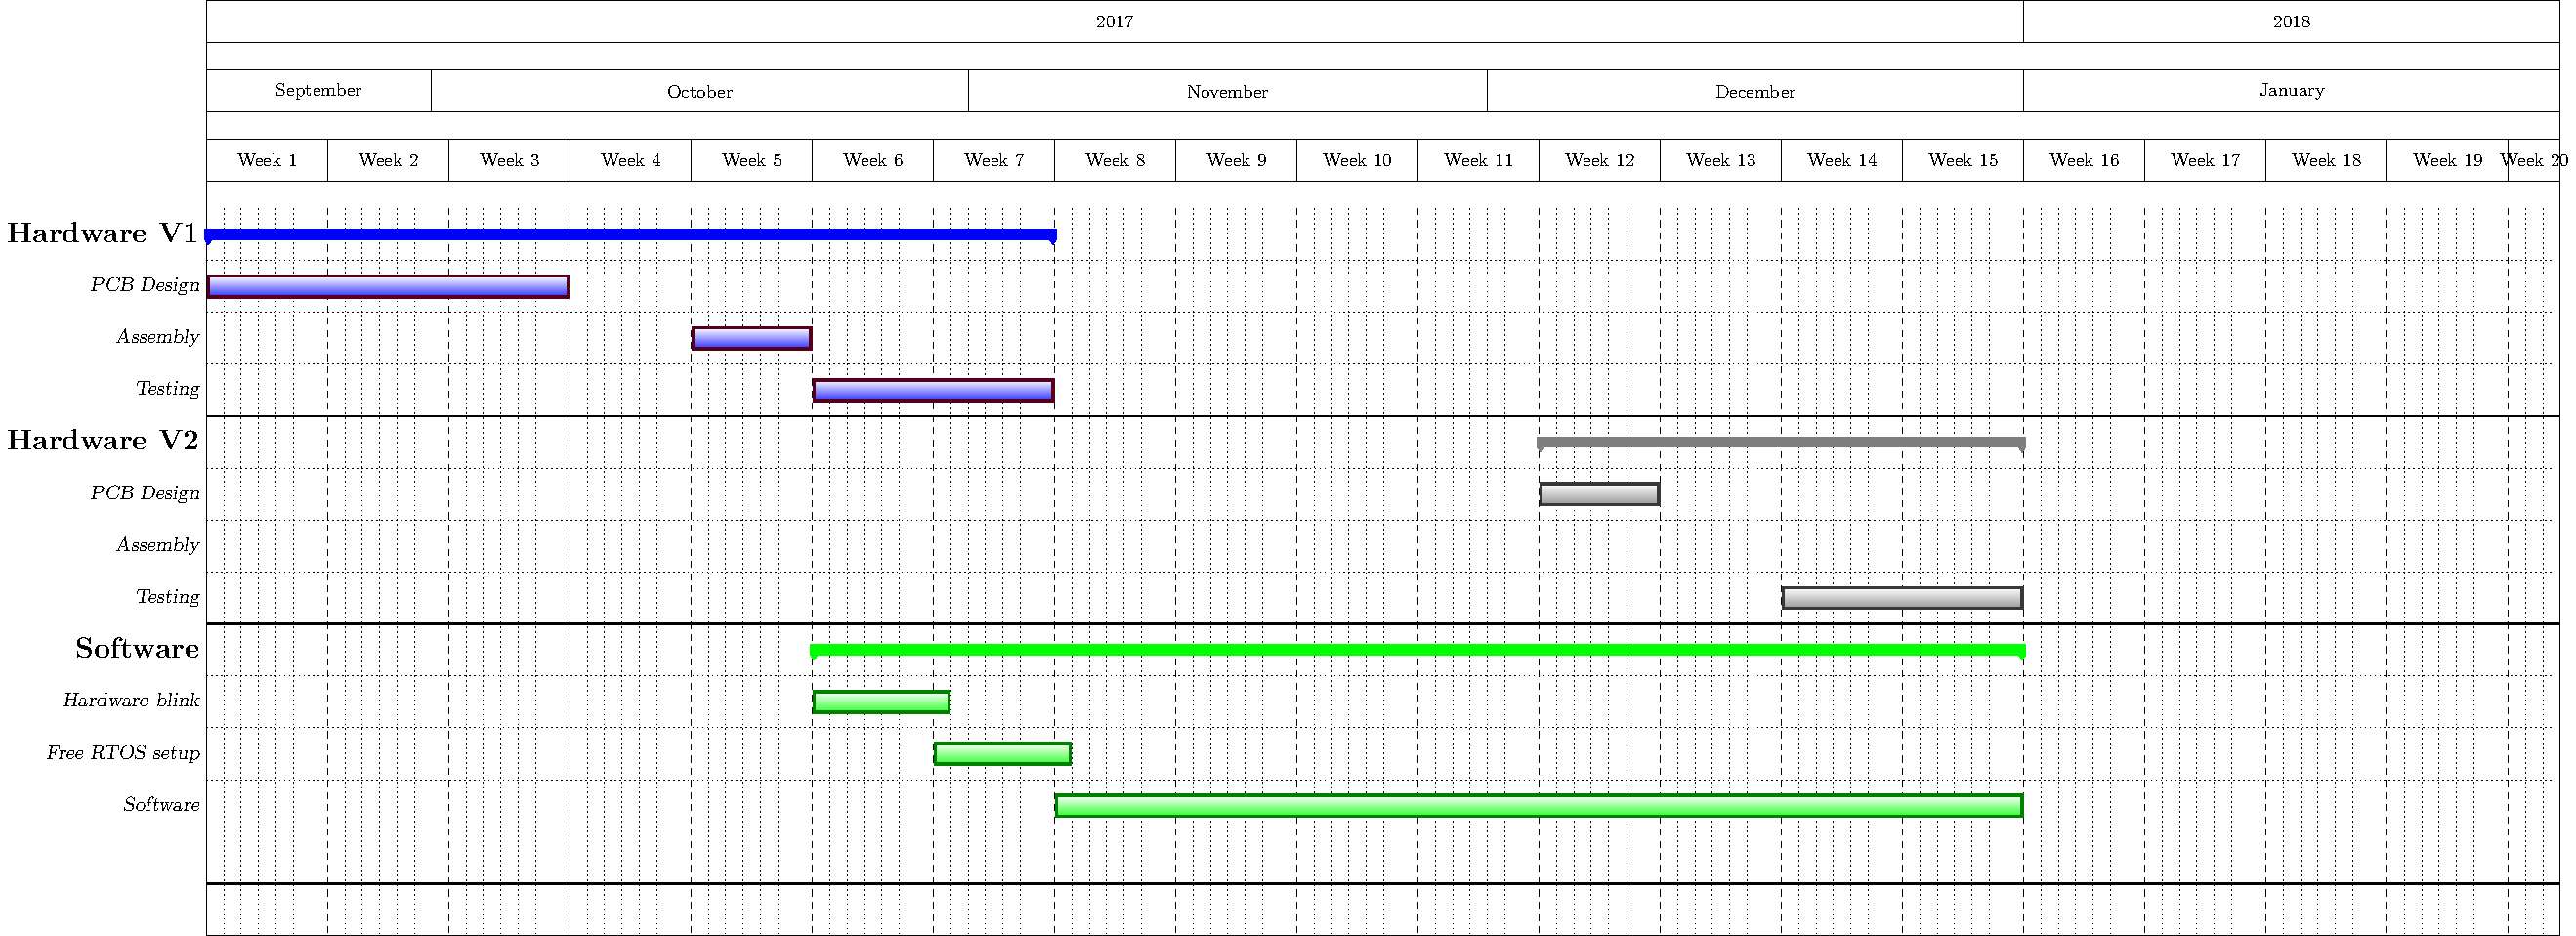
\includegraphics[width=1\textheight, angle=90, origin=c]
    {ProjectPlan_CompleteHwRedesign.pdf}
    \caption{Possible project plan of a complete hardware redesign}
    \label{Project plan complete HW redesign}
\end{figure}
%
\subsection{Adapter Board}
The most profound hardware change is the replacement of the Teensy 3.1.\\
First, a new development board or micro controller has to be selected that supports hardware debugging and meets the requirements for data encryption. \\
After selecting a replacement for the Teensy 3.1, the fastest way to get started with software development for the new micro controller is by designing an adapter board with a Teensy 3.1 footprint. \\
The Teensy 3.1 ships with headers that can be soldered onto the development board. Andreas Albisser designed the interface for the Teensy with female header pins so the development board could simply be plugged into the header and exchanged if needed. This makes it easy to design an adapter print with male headers that match the footprint of the previously used Teensy 3.1. \\
\spic{BareBaseBoard.png}{Base board with female header, Teensy 3.1 not plugged in}{\label{picBareBaseBoard}}
The base board with female headers can be seen in \autoref{picBareBaseBoard}. In this picture, the Teensy 3.1 is not plugged in, the empty headers can be used to route the pins of an other microcontroller to control the base board.\\
This solution has been chosen in the scope of this work to ensure that the end result of this project would provide solid ground work for further development.
%
%
%
\section{Component Evaluation}
Before starting with the design of an adapter board, a replacement for the Teensy 3.1 development board has to be chosen. \\
%
\subsection{Development Board Selection}
The easiest option is to select a more powerful Teensy development board that meets the requirements listed in \todo{Link zu Aufgabenstellung}. \\
Fortunately, both the Teensy 3.5 and Teensy 3.6 meet the requirements and have an on-board SD card slot. A comparison between the Teensies can be found in \autoref{tableTeensyComparison}
%
\begin{table}[h]
    \begin{center}
        \begin{tabular}{l|L{4cm}L{4cm}L{4cm}}
             & \textbf{Teensy 3.1} & \textbf{Teensy 3.5} & \textbf{Teensy 3.6} \\
             \hline
             %-------------------------------------------------------------------------------------
            \textbf{Processor} & MK20DX256 \newline 32 bit ARM \newline Cortex-M4 \newline 72 MHz & 
            MK64FX512VMD12 \newline Cortex-M4F \newline 120 MHz & 
            MK66FX1M0VMD18 \newline Cortex-M4F \newline 180 MHz \\
            \textbf{Flash Memory [bytes]} & 262 k & 512 k & 1024 k \\
            \textbf{RAM Memory [bytes]} & 65 k & 196 k & 256 k \\
            \textbf{EEPROM [bytes]}	 & 2048 & 4096 & 4096 \\
            \textbf{I/O} & 34, 3.3V, 5V tol & 58, 3.3V, 5V tol & 58, 3.3V, 5V tol \\
            \textbf{Analog In} & 21 & 27 & 25 \\
            \textbf{PWM} & 12 & 17 & 19 \\
            \textbf{UART,I2C,SPI} & 3 & 6 & 6 \\
            \textbf{SD Card} & no & yes & yes \\
            \textbf{Price} & \$19.80 & \$25.25 & \$29.25 \\
        \end{tabular}
    \end{center}
    \stabcaption{Teensy comparison}         
    \label{tableTeensyComparison}
\end{table}
%
The pins of both Teensy 3.5 and 3.6 are backwards compatible to the pin out of Teensy 3.1 which will make it easier to develop the PCB of an adapter board. \\
The Teensy 3.5 and Teensy 3.6 development board have all pins needed for SWD hardware debugging available as pads on their backside. \\
The Teensy 3.5 was chosen for this application because there is more support available for this component and an already configured FreeRTOS. This is not the case with the Teensy 3.6.\\
%
%
\subsection{Preparation for Hardware Debugging}
The Teensy development boards are meant for USB programming and debugging. They are equipped with a small micro controller that acts as a boot loader. The small micro controller is in control of the hardware debugging and reset pins of the main micro controller and does the programming of the main micro controller. This way, all Teensies can be used with standard Arduino libraries and programmed with the Arduino IDE. \\
The schematic of the Teensy 3.5 can be seen in \autoref{picSchematicTeensy3.5}. The MKL02Z32VFG4 acts as the boot loader and the MK64FX512 is the main micro controller.\\
\spic{Teensy35_Schematic.png}{Schematic Teensy 3.5}{\label{picSchematicTeensy3.5}}
\spicv{Teensy35_PinAssignment_FrontSide.png}{Pin assignment, front side}{\label{Pin assignment, front side}}{100}
\spicv{Teensy35_PinAssignment_BackSide.png}{Pin assignment, back side}{\label{Pin assignment, back side}}{100}.\\
The pins available to the user are shown in \autoref{Pin assignment, front side} and \autoref{Pin assignment, back side}. \\
%
\subsubsection{Serial Wire Debug (SWD)}
\spicv{SWD_Pinout.png}{SWD pinout}{\label{SWD pinout}}{70}
As can be seen in \autoref{Pin assignment, back side}, there are SWD (Serial Wire Debug) pins are available as pads on the back side of the Teensy 3.5. \\
The SWD interface consists of the following pins:
\begin{itemize}
    \item Vref: Supply voltage
    \item GND: Ground
    \item SWDIO/DD: Debug Data
    \item SWDCLK/DC: Debug Clock
    \item DE: Debug Enable
    \item RST: Reset
\end{itemize}
The physical pinout of a SWD interface can be seen in \autoref{SWD pinout}. Only the reset, data, clock and ground pins are absolutely required to be connected for the debugging interface to work correctly.\\
Both Teensy 3.5 and Teensy 3.6 have the required SWD pins available on their back side but the debug interface is controlled by the on-board boot loader. \\
There are two ways to communicate to the main micro controller directly without the boot loader interfering on the hardware debugging interface:
\begin{itemize}
    \item Holding the boot loader in reset mode.
    \item Removing the boot loader completely.
\end{itemize}
\subsubsection{Resetting the Boot Loader} \label{txtResettingTheBootLoader}
\spic{Pinout_Bootloader.JPG}{Pin out MKL02Z32VFG4}{\label{picPinoutBootLoader}}
According to the data sheet of the boot loader (see \autoref{picPinoutBootLoader} ), pin 15 of the boot loader can have one of three functions: \\
\begin{itemize}
    \item Reset
    \item GPIO input
    \item GPIO output
\end{itemize}
As default, the pin will be configured as a reset pin, but this function can be turned off by configuring it for any of the other two functions in software. \\
Even though the Teensies are fully open source, the software for the boot loader is not available. The only way to find out if the reset pin is still configured as such is by pulling it low and attempting a reset. \\
The location of the boot loader can be found in \autoref{picBootLoaderHighlighted}.\\
Before putting the boot loader into reset mode, any other functions that this micro controller may be responsible for need to be ensured. \\
Because the internal pull ups of the boot loader are used for the reset line of the main micro controller, this reset line needs to be pulled up externally first. \\
\spic{ResettingBootLoader.jpg}{Trying to pull the boot loader into reset mode}{\label{picPullingBootLoaderResetLow}}
A resistor can be soldered onto the Teensy directly for this purpose as seen in \autoref{picPullingBootLoaderResetLow}. Afterwards, pin 15 of the boot loader can be pulled low. \\
Unfortunately, pin 15 seems to be configured as a GPIO pin because pulling the boot loaders reset line low does not prevent it from communicating to the main micro controller of the Teensy 3.5. \\
\spic{Teensy35_uC_keeps_Talking_Even_with_RESET_pulled_to_3V3.png}{The boot loader keeps communicating to the Teensy}{\label{picBootloaderKeepsTalking}}
The state of the hardware debugging pins during idle state were checked with the scope but as can be seen from \autoref{picBootloaderKeepsTalking}, the boot loader is still in control of the debugging interface and therefore the main micro controller.\\
Instead of investigating further into this option, the second option was chosen. \\
%
\subsubsection{Removing the Boot Loader} \label{txtRemovingTheBootLoader}
The MKL02Z32VFG4 has two functions:
\begin{itemize}
    \item It acts as a boot loader and controls the SWD interface to the main micro controller.
    \item It controls the reset line of the main micro controller and its internal pull ups are used to keep the reset line in idle state.
\end{itemize}
To leave the user in full control of the SWD hardware debugging interface, the boot loader has to be removed (or silenced, as attempted in \ref{txtResettingTheBootLoader}). \\
\spicv{BootLoaderHighlighted.png}{Location of the bootloader on Teensy 3.5}{\label{picBootLoaderHighlighted}}{100}
The MKL02Z32VFG4 is located on the front side of the Teensy, as indicated in \autoref{picBootLoaderHighlighted}.\\
\spicv{Teensy35_Modified.png}{Teensy 3.5 modified for hardware debugging}{\label{picModifiedTeensy}}{100}
Flux gel was applied around the boot loader before heating the soldering pads up with hot air to remove the MKL02Z32VFG4. Now a pull up resister was added as seen in \autoref{picModifiedTeensy}. Afterwards, the SWD debugging interface could be used. \\
%
%
%
%
%
%
\section{Teensy Adapter Board}
The design of the adapter board from the footprint of the Teensy 3.1 to the footprint of the Teensy 3.5 was straight forward because of backwards compatibility of the pinout.\\
The Teensy 3.5 is slightly longer than the Teensy 3.1 so the extra pins of the newer version will not be routed down to the main board. The backwards compatible pins can be used like before.\\
Additional components for the adapter board include:
\begin{itemize}
    \item Hardware debugging interface.
    \item Pull up resistor for reset line
    \item Ground header
    \item 3.3V header
\end{itemize}
To prepare the Teensy 3.5 for usage within this project, male headers have to be soldered onto the board and the boot loader has to be removed as in \ref{txtRemovingTheBootLoader}. Because the reset line will be pulled up to 3.3V on the adapter board, the on-board pull up resistor (as seen in \autoref{picModifiedTeensy}) for the reset line is optional. It is only required when working with the Teensy 3.5 stand-alone without the adapter board.\\
Schematic and PCB of the Teensy adapter board can be found in the appendix \todo{Link zum Schema+PCB vom Adapter Board im Appendix}.\\
Issues encountered during development of the adapter board were the pin numbering and interlayer connections.
\subsubsection{Pin numbering}
In a first version of the Teensy adapter board, the pin numbering of the SWD debugging connector was done wrong and had to be adjusted in the footprint for a next PCB version.\\
\spic{DebuggingWithWrongFootprint.jpg}{Hardware debugging with faulty SWD footprint}{\label{picDebugSetupWrongAdapterBoard}}
But instead of waiting for the next PCB version to be produced, all debugging signals were routed manually from the faulty SWD pinout to the debugger. This way, development of the software could be started without delay. A picture of the signal routing can be seen in autoref{picDebugSetupWrongAdapterBoard}.
\subsubsection{Interlayer connections}
The next PCB ordered for internal production at HSLU had poor interlayer connections, most vias did not connect through.\\
To verify the changes on the SWD pinout, the relevant debugging pins were routed manually with small wires and they seem to be correct.\\
But for simplicity and time reasons, not all signals were routed manually but an other order was placed at the HSLU internal production with the hope of better interlayer connections but again with insufficient result.\\
Only on the third HSLU internal order, the inter connection seemed to be satisfying.\\
But by then, there was not enough time to assemble and test the produced adapter boards.\\
%
%
%
%
%
%
%%
%
\chapter{Software}%
% Software
%
A complete documentation of the software written by Andreas Albisser for the Teensy 3.1 can be found in \ref{arduino software analysis}.\\
Various issues found with his software can be found in \ref{Teensy 3.1 software problems}.\\
Now there are two options on how to proceed
\begin{itemize}
    \item Port the existing software to C with FreeRTOS.
    \item Create a new software concept and implement it.
\end{itemize}
Both options are evaluated below.\\
\subsection{Start with existing Software}

%
\section{New Software}%
%
Talk about new SW concept
%
\subsubsection{To-Do List for new SW}%
%
Talk about the things that have not yet been implemented
Package numbering instead of waiting for ACK
No sending out the same package over multiple connections at the same time and only taking the one that was received first.%
%
\chapter{Testing}%
% Testing
%
Testing can be devided into multiple sections:
\begin{itemize}
    \item Testing of hardware
    \item Testing of software 
\end{itemize}
More details about the tests conducted on these items can be found below.
\todo{verifizierung vs verifikation}
%
%
%
%
\section{Hardware Tests} \label{sec:txtHardwareTests}
Testing of the base board was not done in the scope of this project because several fully assembled and tested pieces were provided by Andreas Albisser.\\
Only the Teensy adapter board had to be tested. \\
As seen in \autoref{sec:txtTeensyAdapterBoard}, the first version of the adapter board featured a faulty SWD footprint.\\
The numbering of this footprint was corrected and a new PCB was ordered at the HSLU internal production. The newly produced version had poor interlayer connections and some wires were soldered onto the PCB to verify correctness of the SWD pinout. Because it would have taken up too much time to wire all faulty connections manually, an other order was placed at the HSLU internal production with the hope of better interlayer connections.\\
This time, the vias seemed to be of better quality but there was not enough time to assemble an adapter board to test it out.\\
During the entire project phase, only the first version of the adapter board was available for development and only one board was fully assembled. All software development was therefore done with the setup as in \autoref{fig:picDebugSetupWrongAdapterBoard}.
%
%
%
%
%
\section{Software Tests}
All software was tested against the Teensy 3.1 with the software implementation Andreas Albisser provided. The reason for this being that only one Teensy adapter board has been assembled and the next version that would have been of use was received too late.\\
During and after software development, the functionalities had to be tested. The tests conducted were carried out in the following order:
\begin{itemize}
    \item Echo / loopback
    \item Connecting two UAV Switches directly on wireless side, two serial terminal with USB used on device side
    \item Connecting two UAV Switches with modems on wireless side, two serial terminal with USB used on device side
    \item Connecting two UAV Switches directly on wireless side, autopilot on device side
    \item Connecting two UAV Switches with modems on wireless side, autopilot on device side
\end{itemize}
Not only correct functionality had to be ensured but also system performance:
\begin{itemize}
    \item CPU time of each task
    \item Memory leaks
\end{itemize}
Details about the tests carried out can be found in this chapter.
%
%
%
\subsection{Echo / Loopback} \label{subsec:txtTestLoopback}
The loopback functionality can be enabled with the parameter TEST\_HW\_LOOPBACK\_ONLY in the configuration file located on the SD card.\\
When enabled, all bytes received on each serial connection will be returned on the same serial connection. The main functionality is handled inside the SPI Handler task, both Package Handler and Network Handler tasks will not process any data (but will be running with their configured task interval anyway).
\begin{lstlisting}
vTaskDelayUntil( &lastWakeTime, taskInterval ); /* Wait for the next cycle */
/* read all data and write it to queue */
for(int uartNr = 0; uartNr < NUMBER_OF_UARTS; uartNr++)
{
    /* read data from device spi interface */
    readHwBufAndWriteToQueue(MAX_14830_DEVICE_SIDE, uartNr, RxDeviceBytes[uartNr]);
    /* write data from queue to device spi interface */
    if(config.TestHwLoopbackOnly)
    {
        readQueueAndWriteToHwBuf(MAX_14830_DEVICE_SIDE, uartNr, RxDeviceBytes[uartNr], HW_FIFO_SIZE);
    }
    else
    {
        readQueueAndWriteToHwBuf(MAX_14830_DEVICE_SIDE, uartNr, TxDeviceBytes[uartNr], HW_FIFO_SIZE);
    }
    /* read data from wireless spi interface */
    readHwBufAndWriteToQueue(MAX_14830_WIRELESS_SIDE, uartNr, RxWirelessBytes[uartNr]);
    /* write data from queue to wireless spi interface */
    if(config.TestHwLoopbackOnly)
    {
        readQueueAndWriteToHwBuf(MAX_14830_WIRELESS_SIDE, uartNr, RxWirelessBytes[uartNr], HW_FIFO_SIZE);
    }
    else
    {
        readQueueAndWriteToHwBuf(MAX_14830_WIRELESS_SIDE, uartNr, TxWirelessBytes[uartNr], HW_FIFO_SIZE);
    }
}
\end{lstlisting}
This can be tested easily by connecting the base board with the following configuration to a computer:
\begin{itemize}
    \item TEST\_HW\_LOOPBACK\_ONLY = 1 in configuration file
    \item Set jumper on device side of base board to USB
    \item Connect computer with base board with an USB cable
    \item Open a serial terminal (e.g. Tera Term or PuTTy), select one of the two COM ports that appeared (reminder: the base board has two dual USB to UART converter, see section \autoref{subsec:UsbToUartConverter})
    \item Select the baud rate that was set in the configuration file with the parameter BAUD\_RATES\_DEVICE\_CONN
    \item Turn off local echo on the serial terminal
\end{itemize}
When running the software in Loopback configuration, connecting the device side as an USB COM port, it will look like an echo on the serial terminal in case the local echo is turned off. If local echo is turned on, each character sent will appear twice on the terminal.
%
%
\subsection{Direct Connection of Switches, Tera Term on Device Side} \label{subsec:txtTestDirectConnTeraTerm}
\spic{TestSetupWithTerminal_CableConnection.png}{Setup with direct connection on wireless side, Tera Term on device side}{\label{fig:picCableConnectionAndTeraTerm}}%
Successful package transmission and reception was tested by connecting two UAV Serial Switches directly.\\
Because only one Teensy adapter board was assembled and tested (see \autoref{sec:txtHardwareTests}), the second base board was used with the Teensy 3.1 running with the software developed by Andreas Albisser.\\
The software configuration was as follows:
\begin{itemize}
    \item Set BAUD\_RATES\_WIRELESS\_CONN to the same value on both UAV Serial Switches for the serial interface used
    \item Set jumper on device side of base board to USB
    \item Open a serial terminal (e.g. Tera Term or PuTTy), select one of the two COM ports that appeared (reminder: the base board has two dual USB to UART converter, see section \ref{subsec:UsbToUartConverter})
    \item Turn off local echo on the serial terminal
    \item Select the baud rate that was set in the configuration file with the parameter BAUD\_RATES\_DEVICE\_CONN
    \item Route the used COM port to wireless serial connection 0 with PRIO\_WIRELESS\_CONN\_DEV\_X = 1, 0, 0, 0
    \item Either set a single byte payload mode with USUAL\_PACKET\_SIZE\_DEVICE\_CONN = 1, 0, 0, 0 or set PACKAGE\_GEN\_MAX\_TIMEOUT to a low value (e.g. 5ms) so a package will be generated soon after a single character has been received, no matter how many bytes of payload the package currently holds.
\end{itemize}
%
\subsubsection{No Acknowledge}
First, the software was tested without an acknowledge configured by setting SEND\_ACK\_PER\_WIRELESS\_CONN = 0, 0, 0, 0\\
The software worked as expected. When typing a character on the serial terminal for one UAV Serial Switch, the character appeared at the other terminal and vice versa.
%
\subsubsection{With Acknowledge}
The software was also tested with an acknowledge configured by setting SEND\_ACK\_PER\_WIRELESS\_CONN = 1, 0, 0, 0\\
The software worked as expected. When typing a character on the serial terminal for one UAV Serial Switch, the character appeared at the other terminal and vice versa.
%
%
\subsection{Modem Connection of Switches, Tera Term on Device Side} 
\spic{TestSetupWithTerminal_ModemConnection.png}{Setup with modem connection on wireless side, Tera Term on device side}{\label{fig:picModemConnectionAndTeraTerm}}%
Package handling was also tested by connecting two UAV Serial Switches with modems. The setup was as can be seen in \autoref{fig:picModemConnectionAndTeraTerm}.\\
Because only one Teensy adapter board was assembled and tested (see \autoref{sec:txtHardwareTests}), the second base board was used with the Teensy 3.1 running with the software developed by Andreas Albisser.\\
Device configurations were the same as in \autoref{subsec:txtTestDirectConnTeraTerm}, except for the baud rate on wireless side. The parameter BAUD\_RATES\_WIRELESS\_CONN cannot be chosen freely but has to be set to a value supported by the modem used.\\
The setup was tested with two different modems, one with RS232 interface and the other (RFD900) with a TTL interface where a level converter had to be used to connect modem and wireless side.\\
All modems and hardware used was provided by Aeroscout GmbH. There seemed to be issues with the level converters as they were over heating regularly. This problem  requires further investigation which is outside the scope of this project.
%
\subsubsection{No Acknowledge}
First, the software was tested without an acknowledge configured by setting SEND\_ACK\_PER\_WIRELESS\_CONN = 0, 0, 0, 0\\
The software worked as expected. When typing a character on the serial terminal for one UAV Serial Switch, the character appeared at the other terminal and vice versa.
%
\subsubsection{With Acknowledge}
The software was also tested with an acknowledge configured by setting SEND\_ACK\_PER\_WIRELESS\_CONN = 1, 0, 0, 0\\
The software worked as expected. When typing a character on the serial terminal for one UAV Serial Switch, the character appeared at the other terminal and vice versa.
%
%
\subsection{Direct Connection of Switches, Autopilot on Device Side} \label{subsec:txtTestDirectConnQGroundControl}
To test the system under stress, more data needs to be exchanged between the on-board and the off-board Serial Switch. This is the case when using the system with an autopilot. The hardware used for this test case (QGroundControl and PX4) has been introduced in \autoref{subsec:txtTestResults}.\\
The setup is the same as in \autoref{fig:picQGroundControlCableConnection} but this time with the new software implementation and on the Teensy3.5.\\
Because of a lack of Teensy Adapter Boards, two new software implementation could not be tested against each other. The off-board side always consisted of the base board with a Teensy 3.1.\\
The Serial Switches were configured as follows:
\begin{itemize}
    \item Set jumpers on device side of both base boards to USB
    \item Connect computer with one base board by USB cable and open QGroundControl
    \item Select the baud rate for both Serial Switches that was set in the configuration file with the parameter BAUD\_RATES\_DEVICE\_CONN as configured on pixhawk and QGroundControl (57600 in this case)
    \item Set BAUD\_RATES\_WIRELESS\_CONN to the same value on both UAV Serial Switches for the serial interface used
    \item Set USUAL\_PACKET\_SIZE\_DEVICE\_CONN = 25, 0, 0, 0 and set PACKAGE\_GEN\_MAX\_TIMEOUT to a low value (e.g. 2ms)
    \item Set GENERATE\_DEBUG\_OUTPUT = 1 to enable debug output and the printing interval of the shell to one second by setting THROUGHPUT\_PRINTOUT\_TASK\_INTERVAL = 1
\end{itemize}
%
\subsubsection{No Acknowledge}
\spic{SerialMonitor_Idle_NoAck_QGroundControlConnected.JPG}{QGroundControl in idle mode, no acknowledge configured}{\label{fig:picDebugOutputNoAckIdleMode}}%
The software was tested without an acknowledge configured by setting SEND\_ACK\_PER\_WIRELESS\_CONN = 0, 0, 0, 0\\
First, the PX4 will extablish a connection with QGroundControl. Once the devices have been linked successfully, they will stay in idle mode and less data is exchanged periodically.\\
The connection was established successfully within about 1 second. The amount of data exchanged during connection establishment and during idle mode could be estimated by looking at the debug output on the serial temrinal. The output on the serial terminal during idle mode was as can be seen in \autoref{fig:picDebugOutputNoAckIdleMode}. \\
During idle mode, about 150 bytes/second will be transmitted from PX4 to QGroundControl and about 20 bytes/second will be transmitted from QGroundControl to PX4.\\
From the debug output on the serial terminal during connection establishment, it can be seen that the PX4 transmits around 2500 bytes/second to QGroundControl and receives around 100 bytes/second from QGroundControl.
%
\subsubsection{With Acknowledge}
The software was also tested with acknowledges configured by setting SEND\_ACK\_PER\_WIRELESS\_CONN = 1, 0, 0, 0\\
The software worked as expected. Again, a connection was established successfully within about 1 second and no problems were experienced during idle mode.
%
%
%
%
\subsection{Modem Connection of Switches, Autopilot on Device Side} \label{subsec:txtTestModemtConnQGroundControl}
The system was tested under stress conditions as in \autoref{subsec:txtTestDirectConnQGroundControl} but this time a modem connection instead of directly connected UAV Serial Switches. The setup can be seen in \autoref{fig:picQGroundControlModemConnection}.\\
Software configurations were the same as in \autoref{subsec:txtTestDirectConnQGroundControl}, except for the baud rate on wireless side. The parameter BAUD\_RATES\_WIRELESS\_CONN cannot be chosen freely but has to be set to a value supported by the modem used.\\
The setup was tested with the RS232 modem provided by Aeroscout GmbH.\\
Because of a lack of Teensy Adapter Boards, two new software implementation could not be tested against each other. The off-board side always consisted of the base board with a Teensy 3.1.\\
Tests were conducted with and without acknowledges configured by modifying the configuration parameter SEND\_ACK\_PER\_WIRELESS\_CONN.\\
Due to a lack of time, this test has only been conducted briefly and further time needs to be invested.\\
This test was successful when using the RS232 modem with and without acknowledge configured.\\
The tests were repeated using the RFD900 modem. When no acknowledge was configured, the link establishment successful and took about 2 seconds. When acknowledges were configured, a link could not always be established.\\
%
%
%
%
%
%
%
%
\subsection{System Analysis}
System View is a free tool for system analysis provided by Segger. It reveals runtime behaviour of an application that cannot easily be seen by using a debugger. It provides insight into multi-threading, queues and resource conflicts.\\
There is a processor expert component for System View in Erich Stygers library that makes the usage of this tool very easy. When including this component, it will take care of the communication between the System View software and the developed user application.\\
System View records all queue operations and will display them as events. Because each task performs multiple queue events when called, the processor expert component produces lots of data traffic between System View software and user application when the System View software is active and analyzing. This will result in performance loss of the user application.\\
System View is also limited to capturing one million events for one recording. Because there are many queue operations (which are listed as events), this limit is reached rather quickly.\\
First, the system analysis was done with the processor expert component in its initial state. The software was configured as follows:
\begin{itemize}
    \item Wireless sides were connected directly by wires
    \item Acknowledges were configured
    \item Autopilot running in idle mode, link has already been established
    \item No debug output configured
    \item Shell task interval to a very high and debug output deactivated
\end{itemize}
\spic{SystemView_queueActivated_qGroundControlRunning.JPG}{System View output when queue events captured}{\label{fig:picQueueEventsCaptured}}%
\spic{SystemView_queueDeactivated_qGroundControlRunning_bestCaseSpiHandler.JPG}{System View output when queue events not captured, best case}{\label{fig:picQueueEventsNotCapturedBestCase}}%
\spic{SystemView_queueDeactivated_qGroundControlRunning_worstCaseSpiHandler.JPG}{System View output when queue events not captured, worst case}{\label{fig:picQueueEventsNotCapturedWorstCase}}%
The System View output for this case can be seen in \autoref{fig:picQueueEventsCaptured}. As can be seen in the figure, the SPI Handler takes up most of the CPU time. The SPI Handler task runs for about 2.6 milliseconds, while the Package Handler and the Network Handler task only run for about 0.1 millisecond.\\
But the system performance is affected by the events logged by the System View processor expert component. Deactivating logging of all queue events results in a much better overall system performance. Deactivate logging of queue events can be done by commenting the respective defines out in SEGGER\_SYSTEM\_VIEWER\_FreeRTOS.h:\\
\begin{lstlisting}
//#define traceQUEUE_PEEK( pxQueue )                                    SYSVIEW_RecordU32x4(apiID_OFFSET + apiID_XQUEUEGENERICRECEIVE, SEGGER_SYSVIEW_ShrinkId((U32)pxQueue), SEGGER_SYSVIEW_ShrinkId((U32)pvBuffer), xTicksToWait, xJustPeeking)
//#define traceQUEUE_PEEK_FROM_ISR( pxQueue )                           SEGGER_SYSVIEW_RecordU32x2(apiID_OFFSET + apiID_XQUEUEPEEKFROMISR, SEGGER_SYSVIEW_ShrinkId((U32)pxQueue), SEGGER_SYSVIEW_ShrinkId((U32)pvBuffer))
//#define traceQUEUE_PEEK_FROM_ISR_FAILED( pxQueue )                    SEGGER_SYSVIEW_RecordU32x2(apiID_OFFSET + apiID_XQUEUEPEEKFROMISR, SEGGER_SYSVIEW_ShrinkId((U32)pxQueue), SEGGER_SYSVIEW_ShrinkId((U32)pvBuffer))
//#define traceQUEUE_RECEIVE( pxQueue )                                 SYSVIEW_RecordU32x4(apiID_OFFSET + apiID_XQUEUEGENERICRECEIVE, SEGGER_SYSVIEW_ShrinkId((U32)pxQueue), SEGGER_SYSVIEW_ShrinkId((U32)pvBuffer), xTicksToWait, xJustPeeking)
//#define traceQUEUE_RECEIVE_FAILED( pxQueue )                          SYSVIEW_RecordU32x4(apiID_OFFSET + apiID_XQUEUEGENERICRECEIVE, SEGGER_SYSVIEW_ShrinkId((U32)pxQueue), SEGGER_SYSVIEW_ShrinkId((U32)pvBuffer), xTicksToWait, xJustPeeking)
//#define traceQUEUE_RECEIVE_FROM_ISR( pxQueue )                        SEGGER_SYSVIEW_RecordU32x3(apiID_OFFSET + apiID_XQUEUERECEIVEFROMISR, SEGGER_SYSVIEW_ShrinkId((U32)pxQueue), SEGGER_SYSVIEW_ShrinkId((U32)pvBuffer), (U32)pxHigherPriorityTaskWoken)
//#define traceQUEUE_RECEIVE_FROM_ISR_FAILED( pxQueue )                 SEGGER_SYSVIEW_RecordU32x3(apiID_OFFSET + apiID_XQUEUERECEIVEFROMISR, SEGGER_SYSVIEW_ShrinkId((U32)pxQueue), SEGGER_SYSVIEW_ShrinkId((U32)pvBuffer), (U32)pxHigherPriorityTaskWoken)
#define traceQUEUE_REGISTRY_ADD( xQueue, pcQueueName )                SEGGER_SYSVIEW_RecordU32x2(apiID_OFFSET + apiID_VQUEUEADDTOREGISTRY, SEGGER_SYSVIEW_ShrinkId((U32)xQueue), (U32)pcQueueName)
#if ( configUSE_QUEUE_SETS != 1 )
// #define traceQUEUE_SEND( pxQueue )                                    SYSVIEW_RecordU32x4(apiID_OFFSET + apiID_XQUEUEGENERICSEND, SEGGER_SYSVIEW_ShrinkId((U32)pxQueue), (U32)pvItemToQueue, xTicksToWait, xCopyPosition)
#else
#define traceQUEUE_SEND( pxQueue )                                    SYSVIEW_RecordU32x4(apiID_OFFSET + apiID_XQUEUEGENERICSEND, SEGGER_SYSVIEW_ShrinkId((U32)pxQueue), 0, 0, xCopyPosition)
#endif
#define traceQUEUE_SEND_FAILED( pxQueue )                             SYSVIEW_RecordU32x4(apiID_OFFSET + apiID_XQUEUEGENERICSEND, SEGGER_SYSVIEW_ShrinkId((U32)pxQueue), (U32)pvItemToQueue, xTicksToWait, xCopyPosition)
//#define traceQUEUE_SEND_FROM_ISR( pxQueue )                           SEGGER_SYSVIEW_RecordU32x2(apiID_OFFSET + apiID_XQUEUEGENERICSENDFROMISR, SEGGER_SYSVIEW_ShrinkId((U32)pxQueue), (U32)pxHigherPriorityTaskWoken)
#define traceQUEUE_SEND_FROM_ISR_FAILED( pxQueue )                    SEGGER_SYSVIEW_RecordU32x2(apiID_OFFSET + apiID_XQUEUEGENERICSENDFROMISR, SEGGER_SYSVIEW_ShrinkId((U32)
\end{lstlisting}
Remember that these lines need to be commented out again every time code is generated by the processor expert component.\\
Also, the processor expert component in the library is compatible with the System Viewer version 2.42 while the System Viewer version used is 2.52a. For this reason, some of the events logged inside the System Viewer do not match with the name of the actual event that took place. This does not affect the overall outcome of the system analysis though.\\
Without logging of queue operations, the System View component will generate less traffic. The overall application performance is much better because the tasks take up less CPU time.\\
When the application is running, the CPU time of the SPI Handler fluctuates depending on the amount of data it needs to read from or transmit to the hardware buffer. This can be seen from the System Viewer output. A best case scenario where only little to no data is exchanged between the application and the hardware buffer can be seen in \autoref{fig:picQueueEventsNotCapturedBestCase}. The longest CPU time found during one runtime example can be found in \autoref{fig:picQueueEventsNotCapturedWorstCase}.\\
In best case conditions during idle mode of the autopilot, the SPI Handler task runs for 0.6 milliseconds, the Package Handler and Network Handler tasks both run for 0.05 milliseconds.	\\
In worst case conditions during idle mode of the autopilot, the SPI Handler task runs for 1.9 milliseconds, the Package Handler runs for 0.1 milliseconds and the Network Handler task runs for 0.5 milliseconds.
%
%
%
%
%
%
%
\subsection{Memory Leak}
There are tools to analyze dynamic memory usage such as the Percepio Tracealyzer. Tracelyzer is a real-time visualization tool for RTOS software. There is even a free licence for students in case of non-commercial use.\\
For time reasons, the Tracealyzer has not been installed yet but memory usage has been tested by looking at the free heap available during runtime. The shell offers a command interface for the Free RTOS. There is a command that will display the free heap available to the RTOS. During runtime, this command was run frequently and the heap usage did not change over time, even during stress tests as mentioned in \autoref{subsec:txtTestModemtConnQGroundControl} and \autoref{subsec:txtTestDirectConnQGroundControl}.\\
Many memory leaks have been found at first as there are numerous cases how the software can allocate memory for data but not free it later on. For example memory can be allocated for a package but never freed when the package cannot be pushed onto the queue successfully.%
%
\chapter{Conclusion} \label{sec:txtConclusion}%
% Conclusion
%
The aim of this project was to come up with a flexible application that routes data of connected devices to modems.\\
There was no need to start from scratch for this project as some ground work has been done by Andreas Albisser. He developed a hardware with four RS-232 interfaces to connect data generating and processing devices and four RS-232 interfaces to connect modems for data transmission. The base board has a header to plug in a Teensy 3.2. The Teensy is a small and powerful USB development board that works with Arduino libraries and acts a main micro controller for the base board.\\
The software Andreas Albisser developed for the Teensy 3.2 is complex and not well thought out. Because requirements were added during development, it is hard to maintain and expand.\\
The task description of this project features the use of a more powerful micro controller with Free RTOS as an operating system. Using a different micro controller requires hardware changes. There were two options on how to proceed: either redesign the base board for the new micro controller or design an adapter board that routes the used signals from the new micro controller down to the header of the Teensy 3.2. Because of time reasons, the second option was chosen and an adapter board was designed for the new micro controller used.\\
The Teensy 3.5 was chosen to replace the Teensy 3.2. The Teensy 3.5 features an SD card slot which is also part of the requirements, has more memory and is generally more powerful. Its identical pins are backwards compatible to the pinout of the Teensy 3.2, except for the extra pins because it is slightly longer and has more pins available to the user.\\
The Teensy 3.5 does have hardware debugging pins available on its backside but in order to use them, the on-board bootloader has to be removed as it is in control of the debug pins and cannot be silenced.\\
The hardware debugging pins are routed out on a SWD debug header but the footprint of the header was faulty in the first adapter board version ordered. This mistake was corrected and a second version ordered but the second version had poor inter layer connections. The faulty footprint was tested for correctness and seemed A third version was ordered which is probably better from what can be seen under the microscope. For time reasons, it could not be assembled and tested.\\
Software development was started after the first Teensy Adapter Board had been assembled and the hardware debugging pinout had been corrected manually. First, the software written by Andreas Albisser was analyzed. Because there was almost no documentation available about the software concept or test results, his software concept had to reverse engineered. Because it is complex and hard to expand, a new software concept was drawn up and implemented. The new software concept is according to the ISO/OSI layers and features three main tasks: one for the physical layer (ISO/OSI layer 1), one for the data link layer (ISO/OSI layer 2) and one for the network layer (ISO/OSI layer 3).\\
Layer 1 deals with bytes only and communicates with the hardware components directly. Layer 2 does the assembling of data packages and splits generated data packages into bytes. Layer 3 deals with packages only, their resending in case no acknowledge was received, generates acknowledges for received packages and extracts the payload to push out to the devices connected.\\
Inter task communication is realized with queues, where received data and data to transmit is passed up or down the ISO/OSI layers. All task take the state of all their queues into account during runtime so they will never generate data packages when the queue they should push it to is full. This way, data is never lost intentionally. Currently, each task may lose data unintentionally if a queue operation fails without it being full or empty but for apparently no reason. The only task that will drop data on purpose is the physical layer as it will flush a certain amount of bytes from its queue when full if new data is received and old data has not yet been processed.\\
Generally, the implementation provides about the same functionality as the software developed by Andreas Albisser. The only parameter missing that was part of Andreas' configuration is the limitation of throughput per wireless connection.\\
The base provided by this software is well documented and suitable for further expansion which was not the case with the previous software written for the Teensy 3.2.\\
The next step would be to implement package numbering instead of a system time stamp in the package header. Currently, the receiver does not know about missing packages when looking at the time stamp in the package header because the time stamp is not monotonically increasing. To ensure that packages are always received in the right order, either the sender waits for the acknowledge for a package before sending out the next one or the receiver implements a queue to reassemble packages in their right order before extracting the payload and sending it out to the correct device.\\
Aeroscout GmbH would also like to have data priority configurable. Currently, there is no configuration parameter that allows the user to prioritize one connected device over an other in case of unreliable wireless connection between on-board and off-board Serial Switch.\\
Also, logging has not been implemented yet because of time reasons. The Serial Switch currently prints out debug information on the shell but does not save it in a file.\\
Data encryption and interleaving were part of the task description but have not been implemented yet either.\\
Generally, the aim was of this project was to provide a software that works at least as good as the one provided by Andreas Albisser. Documentation any testing was done at the very end because development of a good and reliable product was prioritized.\\
When testing Andreas Albisser's application with an autopilot software as in a real use-case of Aeroscout GmbH, a connection could not be established successfully when acknowledges were configured for the application and on-board and off-board Serial Switches were communicating wirelessly.\\
When testing the new application with the same autopilot software, a connection was established successfully, even with acknowledges configured and wireless communication between the off-board and on-board devices.\\
Therefore, the goal of this project has been reached because the outcome seems to be of better quality than the state of the project upon start.\\
More time should have been invested into the testing phase to get more detailed results of the project outcome.
%
%
%
%
%
%
%
%
%
\section{Lessons Learned}
This project has been educational in many ways. It was my first time using the operating system Free RTOS and I was struggling during the starting phase because of too many new tools.\\
Also because the start of the project was rather slow and it felt like there was no real progress to show, I was neglecting the documentation up until the very end of the semester. This results in missing pictures in the documentation because they were not taken at that time and missing information because not all the configurations could be remembered when documenting a test case.\\
During the semester, I spent most time working on the project, implementing features and improving performance. This left me with little time for testing at the end where I should have stopped development earlier to invest more time in the testing phase so the person to follow up with this project would know exactly where he/she is at.\\
I do not have a lot of experience with schematics and layouts and did not know about the very high possibility of poor inter layer connections with internally ordered PCBs. Altium Designer together with finding the mistake in the poor inter layer connections cost me a lot of time during this project.\\
Also, I am a first time LaTex user and there were more than one occasion where I remembered Erich Styger's advice: "LaTex without version control is suicide". I can only agree with this statement and am forever glad he mentioned it so early.\\
Last but not least, it will be my goal to always keep the requirements in mind at all times during the next project. It is easy to get lost in coding and adding features. One should always take a step back, look at the requirements and the task description to make sure no element is forgotten. And maybe have a look at the grading paper to see where most time should be invested.%

%--------------------------------------------------------------------------------------------------------------------
% LITERATURVERZEICHNIS
%--------------------------------------------------------------------------------------------------------------------

\literaturverzeichnis%
{true} % LIteraturverzeichnis anzeigen? (true=ja, false=nein)


%--------------------------------------------------------------------------------------------------------------------
% BEZEICHNUNGEN
%--------------------------------------------------------------------------------------------------------------------

\bezeichnungenChapter%
{true} % Bezeichnungen anzeigen? (true=ja, false=nein)
{%b01_Bezeichnungen
%
%
\bezeichnungenSection{true}{ }{
ALOHA & System for coordinating access to a shared communication channel \\
COM port & Simulated serial interface on computer \\
GND & Ground reference, usually 0V\\
HSLU & Lucerne University of Applied Sciences and Arts\\
HW & Hardware\\
ISO/OSI & 7 Layers Model \\
MCU & Micro Controller Unit \\
PC & Personal Computer\\
PCB & Printed Circuit Board\\
RS-232 & Serial interface with +-12V \\
RTT & Real Time Transfer, Segger terminal \\
RTOS & Realtime Operating System \\
RX & Received signal \\
SPI & Serial Peripheral Interface, synchronous communication standard\\
SW & Software\\
SWD & Serial Wire Debug, hardware debugging interface\\
TX & Transmitted signal \\
TTL & Transistor Transistor Level, 5V level\\
UART & Universal Asynchronous Receiver Transmitter \\
UAV & Unmanned Aeral Vehicle \\
USB & Universal Serial Bus
}}



%--------------------------------------------------------------------------------------------------------------------
% ANHANG
%--------------------------------------------------------------------------------------------------------------------

%- - - - - - - - - - - - - - - - - - - - - - - - - - - - - - - - - - - - - - - - - - - - - - - - - - - - - - - - - - 
% outsource_startAppendix
%- - - - - - - - - - - - - - - - - - - - - - - - - - - - - - - - - - - - - - - - - - - - -
\makeatletter 
\def\@makechapterhead#1{
  {\parindent \z@ \raggedright \normalfont
    \interlinepenalty\@M
    \fontsize{16pt}{0pt}\bfseries Anhang \thechapter\quad #1\par\nobreak
    \vskip 60\p@
  }}
\makeatother
%- - - - - - - - - - - - - - - - - - - - - - - - - - - - - - - - - - - - - - - - - - - - -  % Nicht editieren!
%- - - - - - - - - - - - - - - - - - - - - - - - - - - - - - - - - - - - - - - - - - - - - - - - - - - - - - - - - - 

\anhangstuff % Generiert den Anhang-Titel und ändert Spezifikationen
{true} % ist Anhang vorhanden? (true=ja, false=nein)
{
% Anhang content
%
\chapter{Anhangstruktur} \label{refChapterAnhang}%
%
Hier sollte man am besten jegliche Teile über den \textbackslash inlcude-Befehl importieren. Die Überschriften werden genau gleich wie beim Hauptteil des Berichts über die Befehle \textbackslash chapter, \textbackslash section, \textbackslash subsection und \textbackslash subsubsection eingefügt. Die Layoutstruktur ist analog zu den normalen Kapiteln:%
%
\section{Unterkapitel im Anhang} \label{refSectionAnhang}%
%
\blindtext%
%
\subsection{Tieferes Kapitel}%
%
\subsubsection{Noch tieferes Kapitel}%
%
\blindtext%
%
%
%%
}

%- - - - - - - - - - - - - - - - - - - - - - - - - - - - - - - - - - - - - - - - - - - - - - - - - - - - - - - - - - 
% outsource_endAppendix
%- - - - - - - - - - - - - - - - - - - - - - - - - - - - - - - - - - - - - - - - - - - - -
\makeatletter 
\def\@makechapterhead#1{
  {\parindent \z@ \raggedright \normalfont
    \interlinepenalty\@M
    \fontsize{16pt}{0pt}\bfseries \thechapter\quad #1\par\nobreak
    \vskip 60\p@
  }}
\makeatother 
%- - - - - - - - - - - - - - - - - - - - - - - - - - - - - - - - - - - - - - - - - - - - - % Nicht editieren!
%- - - - - - - - - - - - - - - - - - - - - - - - - - - - - - - - - - - - - - - - - - - - - - - - - - - - - - - - - - 


%--------------------------------------------------------------------------------------------------------------------
% LEBENSLAUF (nur in Masterthesis)
%--------------------------------------------------------------------------------------------------------------------
%
%
% Lebenslauf
%
\lebenslauf{true}%
{% Personalien
Name & Peter Muster\\
Adresse & Bahnhofstrasse 1\newline
6004 Luzern\\%
Geburtsdatum & 01.01.1989\\
Heimatort & 6004 Luzern\\
Zivilstand & ledig%
}{% Ausbildung
August 1996 - Juli 2005 & Primar- und Sekundarschule, Dallenwil\\
August 2005 - Juli 2009 & Lehre als Bauzeichner mit technischer Berufsmaturität\newline Biegebruch GmbH, Luzern\\
September 2009 - Juli 2012 & Bauingenieurstudium Bachelor of Science\newline
Hochschule Luzern - Technik \& Architektur, Horw\\
September 2013 - Februar 2016 & Bauingenieurstudium Master of Science\newline
Vertiefung im Konstruktiven Ingenieurbau\newline
Hochschule Luzern - Technik \& Architektur, Horw
}{% Berufliche Tätigkeit
Juli 2010 - August 2010 & Bauzeichner bei Schubversagen AG, Luzern\\
Juli 2011 - August 2011 & Hilfsassistent Abteilung Bautechnik, \newline 
Hochschule Luzern - Technik \& Architektur, Horw \\
Dezember 2012 - September 2015 & Assistent Abteilung Bautechnik,\newline 
Hochschule Luzern - Technik \& Architektur, Horw%
}%
%
%
%--------------------------------------------------------------------------------------------------------------------
% TODO's (nur für Vorabzüge)
%--------------------------------------------------------------------------------------------------------------------

\listoftodos%     % Bei der definitiven Ausgabe des Dokuments auskommentieren

%- - - - - - - - - - - - - - - - - - - - - - - - - - - - - - - - - - - - - - - - - - - - - - - - - - - - - - - - - -  
\end{document} % Nicht editieren!
%- - - - - - - - - - - - - - - - - - - - - - - - - - - - - - - - - - - - - - - - - - - - - - - - - - - - - - - - - - 